\chapter{Filters en overdrachtsfuncties}\label{ch:b1:filters-transfer-functions}

In een luidsprekerkast beslissen een spoel en een condensator, zonder ook maar
één transistor, dat de bas naar de grote conus gaat en de hoge tonen naar de
kleine koepel. De ``AC''-knop van een oscilloscoop verwijdert een traag
driftende offset en houdt de rimpeling erbovenop over. Een voeding maakt van
een kloppende gelijkgerichte netspanning met één condensator een gladde \omterm{def:b1:dc-circuits:voltage}{spanning}.
Alle drie zijn \emph{\omterm{def:b1:filters-transfer-functions:H}{filters}}: \omterm{def:b1:dc-circuits:linear}{lineaire netwerken} die elke frequentie
anders behandelen. Omdat elk periodiek \omterm{def:b1:wave-propagation:signal}{signaal} een som van sinussen is, is weten
wat een schakeling met elke sinus doet --- haar \omterm{def:b1:filters-transfer-functions:H}{overdrachtsfunctie} --- weten
wat zij met alles doet. Dit hoofdstuk definieert \omterm{def:b1:filters-transfer-functions:H}{overdrachtsfuncties}, tekent
hun bodediagrammen voor de schakelingen van eerste en tweede orde uit de vorige
hoofdstukken, en gebruikt ze om te voorspellen hoe een blokgolf uit een \omterm{def:b1:filters-transfer-functions:H}{filter}
komt.

\section{Overdrachtsfunctie en bodediagram}

\begin{definition}[Overdrachtsfunctie]\label{def:b1:filters-transfer-functions:H}
\index{overdrachtsfunctie}\index{versterking}\index{filter}
Een \omterm{def:b1:dc-circuits:linear}{lineair netwerk} met een ingangsspanning $\underline U_e$ en een
uitgangsspanning $\underline U_s$ (gemeten met niets aan de uitgang) heeft
de \emph{overdrachtsfunctie}
\[
\underline H(j\omega) = \frac{\underline U_s}{\underline U_e},
\qquad G(\omega) = \abs{\underline H}, \qquad \varphi(\omega) = \arg\underline H,
\]
met de \emph{versterking} $G$ (verhouding van de \omterm{def:b1:wave-propagation:signal}{amplitudes}) en de faseverschuiving $\varphi$
van de uitgang ten opzichte van de ingang. Een \emph{filter} is zo'n netwerk
dat om zijn frequentieafhankelijkheid wordt gebruikt: een sinus met \omterm{def:b1:wave-propagation:signal}{amplitude} $E$ bij
$\omega$ komt eruit als $G(\omega)E\cos(\omega t + \varphi(\omega))$.
\end{definition}

\begin{definition}[Decibel; bodediagram]\label{def:b1:filters-transfer-functions:bode}
\index{decibel}\index{bodediagram}\index{afsnijfrequentie}\index{doorlaatband}
De \omterm{def:b1:filters-transfer-functions:H}{versterking} in \emph{decibel} is $G_{\mathrm{dB}} = 20\log_{10}G$: een factor
$10$ is \qty{20}{dB}, een factor $2$ is \qty{6}{dB} en $1/\sqrt2$ is
\qty{-3}{dB}. Het \emph{bodediagram} zet $G_{\mathrm{dB}}$ en
$\varphi$ uit tegen $\log_{10}\omega$ (of $f$). De \emph{afsnijfrequentie}
is waar $G$ tot $G_{\max}/\sqrt2$ daalt (\qty{-3}{dB} onder
het maximum); de \emph{doorlaatband} is het frequentiegebied binnen
\qty{3}{dB} van het maximum. Een decade is een factor $10$ in frequentie, een
octaaf een factor $2$.
\end{definition}

\begin{method}[De aard van een filter in één oogopslag]\label{met:b1:filters-transfer-functions:nature}
Kijk vóór het rekenen naar de limieten: bij zeer lage frequentie is een condensator
een open keten en een spoel een draad; bij zeer hoge frequentie precies
andersom. Vervang beide en lees af of de uitgang de ingang is
(doorgelaten) of nul (geblokkeerd). Laat laag door, blokkeert hoog: laagdoorlaat; het
omgekeerde: hoogdoorlaat; blokkeert beide: banddoorlaat; laat beide door: bandsper.
Bereken daarna $\underline H$ met een \omterm{prop:b1:dc-circuits:dividers}{spanningsdeler}.
\end{method}

\section{Filters van de eerste orde}

\begin{proposition}[Laagdoorlaatfilter van de eerste orde]\label{prop:b1:filters-transfer-functions:lowpass1}
\index{laagdoorlaatfilter}\index{integrator}
De RC-deler met de uitgang over $C$ (of de RL-deler met de uitgang
over $R$) heeft
\[
\underline H = \frac{1}{1 + j\omega/\omega_c}, \qquad
\omega_c = \frac{1}{RC} \ \Big(\text{of } \frac{R}{L}\Big),
\qquad G = \frac{1}{\sqrt{1 + (\omega/\omega_c)^2}}, \qquad
\varphi = -\arctan\frac{\omega}{\omega_c} .
\]
Bode-asymptoten: $G_{\mathrm{dB}} = 0$ voor $\omega \ll \omega_c$, en een
rechte die \qty{20}{dB} per decade daalt voor $\omega \gg \omega_c$;
zij snijden elkaar in $\omega_c$, waar de echte kromme \qty{-3}{dB} is en
$\varphi = -45^\circ$. Voor $\omega \gg \omega_c$ is $\underline H \approx
\omega_c/(j\omega)$: de uitgang is evenredig met de \emph{integraal}
van de ingang --- daar is het \omterm{def:b1:filters-transfer-functions:H}{filter} een integrator.
\end{proposition}

\begin{proof}
\omterm{prop:b1:dc-circuits:dividers}{Spanningsdeler}:
\[
\underline H = \frac{1/jC\omega}{R + 1/jC\omega} = \frac{1}{1 + jRC\omega} .
\]
Ver boven de \omterm{def:b1:filters-transfer-functions:bode}{afsnijfrequentie} is $1 + j\omega/\omega_c \approx j\omega/\omega_c$, en
een \omterm{def:b1:sinusoidal-impedance:complex}{complexe amplitude} door $j\omega$ delen is integreren
(\cref{prop:b1:sinusoidal-impedance:rules}): $u_s \approx \omega_c\int u_e\,\dd t$.
$20\log(\omega_c/\omega)$ verliest \qty{20}{dB} per vertienvoudiging van $\omega$.
\end{proof}

\begin{proposition}[Hoogdoorlaatfilter van de eerste orde]\label{prop:b1:filters-transfer-functions:highpass1}
\index{hoogdoorlaatfilter}\index{differentiator}
De CR-deler met de uitgang over $R$ (of LR met de uitgang over $L$)
heeft
\[
\underline H = \frac{j\omega/\omega_c}{1 + j\omega/\omega_c},
\qquad G = \frac{\omega/\omega_c}{\sqrt{1 + (\omega/\omega_c)^2}},
\qquad \varphi = \frac{\pi}{2} - \arctan\frac{\omega}{\omega_c},
\]
stijgend met \qty{20}{dB} per decade onder $\omega_c$, vlak erboven, \qty{-3}{dB}
en $+45^\circ$ bij $\omega_c$. Voor $\omega \ll \omega_c$ is $\underline H
\approx j\omega/\omega_c$: de uitgang is evenredig met de
\emph{afgeleide} van de ingang.
\end{proposition}

\begin{proof}
$\underline H = R/(R + 1/jC\omega) = jRC\omega/(1 + jRC\omega)$;
met $j\omega$ vermenigvuldigen is differentiëren.
\end{proof}

\begin{omfigure}
\begin{tikzpicture}
\begin{axis}[omaxis, axis x line=bottom, axis y line=left, xlabel style={at={(axis description cs:0.5,-0.14)}, anchor=north}, width=7.4cm, height=5.2cm, xmode=log, xlabel={$\omega/\omega_c$},
    ylabel={$G_{\mathrm{dB}}$}, xmin=0.01, xmax=100, ymin=-42, ymax=6,
    ytick={0,-20,-40}, yticklabels={$0$,$-20$,$-40$},
    xtick={0.01,0.1,1,10,100}, xticklabels={$10^{-2}$,$10^{-1}$,$1$,$10$,$10^{2}$}]
  \addplot[omExo, dashed, domain=0.01:1, samples=2] {0};
  \addplot[omExo, dotted, domain=0.01:100, samples=2] {-3};
  \addplot[omExo, dashed, domain=1:100, samples=2] {-20*log10(x)};
  \addplot[omDef, thick, domain=0.01:100, samples=200] {-10*log10(1 + x^2)};
  \addplot[omThm, thick, domain=0.01:100, samples=200] {-10*log10(1 + 1/x^2)};
  \node[omDef, font=\footnotesize] at (axis cs:0.05,-7) {laagdoorlaat};
  \node[omThm, font=\footnotesize] at (axis cs:30,-9) {hoogdoorlaat};
\end{axis}
\end{tikzpicture}\qquad
\begin{tikzpicture}
\begin{axis}[omaxis, axis x line=bottom, axis y line=left, xlabel style={at={(axis description cs:0.5,-0.14)}, anchor=north}, width=7.0cm, height=5.2cm, xmode=log, xlabel={$\omega/\omega_c$},
    ylabel={$\varphi$}, xmin=0.01, xmax=100, ymin=-1.8, ymax=1.8,
    ytick={-1.5708,-0.7854,0,0.7854,1.5708}, yticklabels={$-\frac{\pi}{2}$,$-\frac{\pi}{4}$,$0$,$\frac{\pi}{4}$,$\frac{\pi}{2}$},
    xtick={0.01,0.1,1,10,100}, xticklabels={$10^{-2}$,$10^{-1}$,$1$,$10$,$10^{2}$}]
  \addplot[omDef, thick, domain=0.01:100, samples=200] {-rad(atan(x))};
  \addplot[omThm, thick, domain=0.01:100, samples=200] {rad(90 - atan(x))};
\end{axis}
\end{tikzpicture}

{\small Bodediagrammen van het laagdoorlaatfilter (blauw) en het
\omterm{prop:b1:filters-transfer-functions:highpass1}{hoogdoorlaatfilter} (rood) van de eerste orde: de \omterm{def:b1:filters-transfer-functions:H}{versterking} in \omterm{def:b1:filters-transfer-functions:bode}{decibel} met de
asymptoten (streepjes) die elkaar bij de \omterm{def:b1:filters-transfer-functions:bode}{afsnijfrequentie} snijden, waar de
echte \omterm{def:b1:filters-transfer-functions:H}{versterking} \qty{-3}{dB} is, en de fase, die daar $\mp45^\circ$ passeert.}
\end{omfigure}

\begin{example}[AC-koppeling]\label{ex:b1:filters-transfer-functions:accoupling}
De AC-ingang van een oscilloscoop is een \omterm{prop:b1:filters-transfer-functions:highpass1}{hoogdoorlaatfilter} met $f_c \approx \qty{10}{Hz}$:
een \omterm{def:b1:wave-propagation:signal}{signaal} van \qty{1}{kHz} boven op een offset van \qty{5}{V} komt door bij
\qty{-0.0002}{dB} en zonder die offset. Maar een blokgolf van \qty{50}{Hz}
wordt zichtbaar vervormd --- haar vlakke toppen zakken weg --- omdat het \omterm{def:b1:filters-transfer-functions:H}{filter}
bij \qty{50}{Hz} maar één decade boven zijn \omterm{def:b1:filters-transfer-functions:bode}{afsnijfrequentie} zit en de lage
harmonischen van het \omterm{def:b1:wave-propagation:signal}{signaal} in fase worden verschoven
(\cref{exo:b1:filters-transfer-functions:12}).
\end{example}

\section{Filters van de tweede orde}

\begin{proposition}[De RLC in serie als drie filters]\label{prop:b1:filters-transfer-functions:rlc}
\index{banddoorlaatfilter}\index{filter van de tweede orde}
Met $x = \omega/\omega_0$, $\omega_0 = 1/\sqrt{LC}$ en $Q =
\sqrt{L/C}/R$ geeft de RLC in serie, gevoed door $\underline U_e$, naargelang
waar de uitgang wordt genomen:
\begin{align*}
\text{over } C:&\quad \underline H = \frac{1}{1 - x^2 + jx/Q}, \\
\text{over } R:&\quad \underline H = \frac{jx/Q}{1 - x^2 + jx/Q} = \frac{1}{1 + jQ(x - 1/x)}, \\
\text{over } L:&\quad \underline H = \frac{-x^2}{1 - x^2 + jx/Q}:
\end{align*}
een laagdoorlaat-, een banddoorlaat- en een \omterm{prop:b1:filters-transfer-functions:highpass1}{hoogdoorlaatfilter} van de tweede orde. Ver van
$\omega_0$ vallen het laag- en het \omterm{prop:b1:filters-transfer-functions:highpass1}{hoogdoorlaatfilter} met \qty{40}{dB} per decade,
het banddoorlaatfilter met \qty{20}{dB} per decade aan elke kant; het banddoorlaatfilter
heeft zijn maximum $1$ bij $\omega_0$ en de bandbreedte $\Delta\omega =
\omega_0/Q$ uit \cref{thm:b1:sinusoidal-impedance:resonance}.
\end{proposition}

\begin{proof}
\omterm{prop:b1:dc-circuits:dividers}{Spanningsdelers} met de totale \omterm{def:b1:sinusoidal-impedance:impedance}{impedantie} $R + j(L\omega - 1/C\omega)$;
vermenigvuldig teller en noemer met $jC\omega$ en gebruik
$LC\omega_0^2 = 1$, $RC\omega_0 = 1/Q$. Het banddoorlaatfilter is de
stroomresonantie van het vorige hoofdstuk, gelezen als \omterm{def:b1:dc-circuits:voltage}{spanning} over $R$.
\end{proof}

\begin{proposition}[Laagdoorlaat van de tweede orde: de rol van $Q$]\label{prop:b1:filters-transfer-functions:lowpass2}
\index{resonantie!van een filter}
Voor het laagdoorlaatfilter is $G = 1/\sqrt{(1 - x^2)^2 + x^2/Q^2}$: voor
$Q > 1/\sqrt2$ stijgt de \omterm{def:b1:filters-transfer-functions:H}{versterking} boven $1$ in de buurt van $\omega_0$ (resonantie, piek
$\approx Q$ voor grote $Q$); voor $Q = 1/\sqrt2$ is zij ``maximaal vlak'',
$G = 1/\sqrt{1 + x^4}$, precies \qty{-3}{dB} bij $\omega_0$; voor kleinere
$Q$ zakt zij vroeg weg. De fase loopt van $0$ tot $-\pi$, en passeert $-\pi/2$
bij $\omega_0$.
\end{proposition}

\begin{proof}
$(1 - x^2)^2 + x^2/Q^2 = 1 + x^4 + x^2(1/Q^2 - 2)$: de middelste term
verdwijnt voor $Q^2 = \tfrac12$, is negatief (piek) daarboven en positief
(wegzakken) daaronder; het gedrag rond $x = 1$ is geanalyseerd in
\cref{prop:b1:sinusoidal-impedance:overvoltage}.
\end{proof}

\begin{omfigure}
\begin{tikzpicture}
\begin{axis}[omaxis, axis x line=bottom, axis y line=left, xlabel style={at={(axis description cs:0.5,-0.14)}, anchor=north}, width=7.4cm, height=5.4cm, xmode=log, xlabel={$\omega/\omega_0$},
    ylabel={$G_{\mathrm{dB}}$}, xmin=0.1, xmax=10, ymin=-45, ymax=15,
    ytick={10,0,-20,-40}, xtick={0.1,1,10}, xticklabels={$0.1$,$1$,$10$},
    legend style={at={(0.03,0.03)}, anchor=south west, font=\footnotesize, draw=none, fill=none}]
  \addplot[omDef, thick, domain=0.1:10, samples=300] {-10*log10((1 - x^2)^2 + x^2/9)};
  \addlegendentry{$Q = 3$}
  \addplot[omThm, thick, domain=0.1:10, samples=300] {-10*log10(1 + x^4)};
  \addlegendentry{$Q = 1/\sqrt2$}
  \addplot[omProp, thick, domain=0.1:10, samples=300] {-10*log10((1 - x^2)^2 + x^2/0.04)};
  \addlegendentry{$Q = 0.2$}
  \addplot[omExo, dashed, domain=1:10, samples=2] {-40*log10(x)};
\end{axis}
\end{tikzpicture}\qquad
\begin{tikzpicture}
\begin{axis}[omaxis, axis x line=bottom, axis y line=left, xlabel style={at={(axis description cs:0.5,-0.14)}, anchor=north}, width=7.0cm, height=5.4cm, xmode=log, xlabel={$\omega/\omega_0$},
    ylabel={$G_{\mathrm{dB}}$}, xmin=0.1, xmax=10, ymin=-45, ymax=5,
    ytick={0,-20,-40}, xtick={0.1,1,10}, xticklabels={$0.1$,$1$,$10$},
    legend style={at={(0.03,0.97)}, anchor=north west, font=\footnotesize, draw=none, fill=none}]
  \addplot[omExo, dotted, domain=0.1:10, samples=2, forget plot] {-3};
  \addplot[omDef, thick, domain=0.1:10, samples=400] {-10*log10(1 + 100*(x - 1/x)^2)};
  \addlegendentry{$Q = 10$}
  \addplot[omThm, thick, domain=0.1:10, samples=300] {-10*log10(1 + (x - 1/x)^2)};
  \addlegendentry{$Q = 1$}
\end{axis}
\end{tikzpicture}

{\small \omterm{def:b1:filters-transfer-functions:H}{Filters} van de tweede orde uit de RLC in serie. Links het laagdoorlaatfilter
(uitgang over $C$) voor drie waarden van $Q$: een resonantiepiek, het maximaal
vlakke antwoord of een vroeg wegzakken, alle uitkomend op de asymptoot van
\qty{-40}{dB/decade} (streepjes). Rechts het banddoorlaatfilter (uitgang over $R$): een piek
met breedte $\omega_0/Q$ die aan elke kant \qty{20}{dB/decade} daalt.}
\end{omfigure}

\begin{example}[Een wisselfilter]\label{ex:b1:filters-transfer-functions:crossover}
De woofer en de tweeter van een luidspreker, elk \qty{8}{\ohm}, delen de
versterker via een laagdoorlaatfilter (een spoel in serie) en een
\omterm{prop:b1:filters-transfer-functions:highpass1}{hoogdoorlaatfilter} (een condensator in serie), afgesneden bij \qty{2}{kHz}: $L = R/\omega_c = \qty{0.64}{mH}$,
$C = 1/R\omega_c = \qty{10}{\micro F}$. Bij \qty{2}{kHz} krijgt elke eenheid
\qty{-3}{dB}, dus het halve vermogen, en geldt $G_L^2 + G_H^2 = 1$ bij elke
frequentie: het vermogen wordt verdeeld, niet verspild. De weekendopgave ontwerpt
een steilere versie.
\end{example}

\section{Een periodiek signaal filteren}

\begin{theorem}[Fourierontbinding]\label{thm:b1:filters-transfer-functions:fourier}
\index{fourierreeks}\index{harmonische}\index{spectrum!van een periodiek signaal}
Een periodiek \omterm{def:b1:wave-propagation:signal}{signaal} met periode $T = 2\pi/\omega$ (redelijk regelmatig) is
de som van een constante en van sinussen bij de veelvouden van $\omega$:
\[
s(t) = c_0 + \sum_{n = 1}^{\infty} c_n\cos(n\omega t + \varphi_n),
\]
waarin $c_0 = \langle s\rangle$ de gemiddelde waarde is; de term $n = 1$ is
de \emph{grondtoon}, de overige zijn de \emph{harmonischen}, en de
\omterm{def:b1:wave-propagation:signal}{amplitudes} $c_n$ vormen het \emph{spectrum}. Een blokgolf met \omterm{def:b1:wave-propagation:signal}{amplitude}
$\pm E$ heeft $c_n = 4E/(n\pi)$ voor oneven $n$ en $0$ voor even $n$; een
driehoeksgolf met \omterm{def:b1:wave-propagation:signal}{amplitude} $\pm E$ heeft $c_n = 8E/(n\pi)^2$ voor oneven $n$.
\end{theorem}
\admitted

\begin{remark}[Wat je eraan hebt]\label{rem:b1:filters-transfer-functions:fourier}
De stelling en de berekening van de $c_n$ horen bij de wiskunde van
jaar 2. Hier is zij een gereedschap: scherpe hoeken vragen veel
harmonischen (die van de blokgolf nemen maar af als $1/n$), gladde signalen
vragen er weinig (die van de driehoek als $1/n^2$). De harmonische inhoud van een
\omterm{def:b1:wave-propagation:signal}{signaal} is waar de klankkleur van een instrument uit bestaat, en waarop een \omterm{def:b1:filters-transfer-functions:H}{filter} inwerkt.
\end{remark}

\begin{proposition}[Lineair filteren van een periodiek signaal]\label{prop:b1:filters-transfer-functions:filtering}
Door een \omterm{def:b1:filters-transfer-functions:H}{filter} met \omterm{def:b1:filters-transfer-functions:H}{overdrachtsfunctie} $\underline H$ wordt het \omterm{def:b1:wave-propagation:signal}{signaal} uit de
stelling
\[
s_{\text{uit}}(t) = G(0)\,c_0 + \sum_{n \geq 1} G(n\omega)\,c_n\cos\!\big(n\omega t + \varphi_n + \varphi(n\omega)\big):
\]
elke harmonische wordt geschaald met de \omterm{def:b1:filters-transfer-functions:H}{versterking} en verschoven met de fase bij
\emph{haar eigen} frequentie, en daarna worden de stukken opgeteld. Dus:
\begin{itemize}
  \item een laagdoorlaatfilter met $\omega_c \ll \omega$ houdt in wezen $c_0$ over:
        het \emph{middelt} (gladstrijken, rimpel wegnemen) en maakt van een
        blokgolf een kleine driehoek (integratie);
  \item een \omterm{prop:b1:filters-transfer-functions:highpass1}{hoogdoorlaatfilter} met $\omega_c \ll \omega$ haalt $c_0$ weg en laat
        de rest door (AC-koppeling); met $\omega_c \gg \omega$
        differentieert het (pieken bij de flanken van een blokgolf);
  \item een banddoorlaatfilter afgestemd op $n\omega$ met $Q \gg 1$ haalt de
        $n$-de harmonische er alleen uit: een sinus uit een blokgolf.
\end{itemize}
\end{proposition}

\begin{proof}
Superpositie voor een \omterm{def:b1:dc-circuits:linear}{lineair netwerk} (\cref{thm:b1:dc-circuits:superposition})
toegepast op de som van sinusvormige ingangen, elk behandeld met
\cref{def:b1:filters-transfer-functions:H}.
\end{proof}

\begin{omfigure}
\begin{tikzpicture}
\begin{axis}[omaxis, axis x line=bottom, width=6.6cm, height=4.8cm, xlabel={harmonische $n$}, ylabel={$c_n/c_1$},
    xmin=0, xmax=10, ymin=0, ymax=1.15, xtick={1,3,5,7,9}, ytick={0.5,1}]
  \addplot[ybar, bar width=7pt, fill=omDef!35, draw=omDef] coordinates {(1,1) (3,0.333) (5,0.2) (7,0.143) (9,0.111)};
  \addplot[ybar, bar width=3.5pt, fill=omThm, draw=omThm] coordinates
    {(1,0.7071) (3,0.1054) (5,0.0392) (7,0.0202) (9,0.0123)};
  \node[omDef, font=\footnotesize] at (axis cs:6.0,0.9) {blokgolf (blauw)};
  \node[omThm, font=\footnotesize] at (axis cs:6.0,0.7) {na laagdoorlaat (rood)};
\end{axis}
\end{tikzpicture}\hfill
\begin{tikzpicture}
\begin{axis}[omaxis, axis x line=bottom, width=6.6cm, height=4.8cm, xlabel={$t/T$}, ylabel={$u$},
    xmin=0, xmax=2, ymin=-1.3, ymax=1.3, xtick={0.5,1,1.5,2}, ytick={-1,1}, yticklabels={$-E$,$E$}]
  % square wave
  \addplot[omDef!60, thick, const plot, domain=0:2, samples=5] coordinates {(0,1) (0.5,-1) (1,1) (1.5,-1) (2,-1)};
  % RC response with tau = T/(2pi) (wc = w): on each half period u = s + (u0 - s) e^{-t/tau}; steady amplitude A = tanh(T/(4 tau)) = tanh(pi/2)=0.917
  \addplot[omThm, thick, domain=0:0.5, samples=60] {1 - (1 + 0.917)*exp(-2*pi*x)};
  \addplot[omThm, thick, domain=0.5:1, samples=60] {-1 + (1 + 0.917)*exp(-2*pi*(x-0.5))};
  \addplot[omThm, thick, domain=1:1.5, samples=60] {1 - (1 + 0.917)*exp(-2*pi*(x-1))};
  \addplot[omThm, thick, domain=1.5:2, samples=60] {-1 + (1 + 0.917)*exp(-2*pi*(x-1.5))};
  % tau = T/(20 pi): wc = 10 w: amplitude tanh(5 pi)=1
  \addplot[omProp, thick, domain=0:0.5, samples=80] {1 - 2*exp(-20*pi*x)};
  \addplot[omProp, thick, domain=0.5:1, samples=80] {-1 + 2*exp(-20*pi*(x-0.5))};
  \addplot[omProp, thick, domain=1:1.5, samples=80] {1 - 2*exp(-20*pi*(x-1))};
  \addplot[omProp, thick, domain=1.5:2, samples=80] {-1 + 2*exp(-20*pi*(x-1.5))};
\end{axis}
\end{tikzpicture}

{\small Een blokgolf door een laagdoorlaatfilter van de eerste orde. Links haar
spectrum (oneven harmonischen als $1/n$) en het spectrum na een \omterm{def:b1:filters-transfer-functions:H}{filter} dat bij
de grondtoon afsnijdt. Rechts het tijdsignaal voor $\omega_c = \omega$ (rood,
exponentiële bogen) en $\omega_c = 10\omega$ (oranje, alleen afgeronde
hoeken); met $\omega_c \ll \omega$ zou de uitgang een kleine driehoek rond
het gemiddelde zijn.}
\end{omfigure}

\begin{example}[Getallen]\label{ex:b1:filters-transfer-functions:numbers}
Een blokgolf van \qty{1}{kHz} met \omterm{def:b1:wave-propagation:signal}{amplitude} \qty{5}{V}: harmonischen van
\qty{6.37}{V} bij \qty{1}{kHz}, \qty{2.12}{V} bij \qty{3}{kHz},
\qty{1.27}{V} bij \qty{5}{kHz}. Door een RC-laagdoorlaat afgesneden bij
\qty{10}{Hz} ($\tau = \qty{16}{ms}$) is de uitgang een driehoek met
\omterm{def:b1:wave-propagation:signal}{amplitude} $ET/4\tau \approx \qty{80}{mV}$ rond nul; door een
banddoorlaat afgestemd op \qty{3}{kHz} met $Q = 20$ een sinus van \qty{2.1}{V}
bij \qty{3}{kHz} met slechts enkele procenten van de buren
(\cref{exo:b1:filters-transfer-functions:8}).
\end{example}

\section{Filters in cascade}

\begin{proposition}[Cascade en belasting]\label{prop:b1:filters-transfer-functions:cascade}
\index{cascade (van filters)}\index{belasting (van een filter)}
Twee \omterm{def:b1:filters-transfer-functions:H}{filters} in cascade hebben $\underline H = \underline H_1\underline H_2$
--- de \omterm{def:b1:filters-transfer-functions:H}{versterkingen} vermenigvuldigen, de \omterm{def:b1:filters-transfer-functions:bode}{decibels} en fasen tellen op --- \emph{mits het
tweede het eerste niet belast}, dus verwaarloosbaar weinig stroom uit zijn
uitgang trekt. Anders moeten de delerbetrekkingen voor het samengestelde
netwerk opnieuw worden opgeschreven. Een volger met operationele versterker
(\cref{ch:b1:operational-amplifier}) tussen de trappen maakt de productregel
exact.
\end{proposition}

\begin{proof}
$\underline H_1$ is gedefinieerd met een open uitgang; is de ingangsimpedantie
van de volgende trap veel groter dan de uitgangsimpedantie van de eerste
(haar Thévenin-weerstand), dan blijft de uitgangsspanning onveranderd en ziet de
tweede trap precies $\underline U_{s1}$ als ingang.
\end{proof}

\begin{example}[Twee RC-trappen]\label{ex:b1:filters-transfer-functions:tworc}
Twee gelijke RC-laagdoorlaatfilters achter elkaar geven \emph{niet}
$1/(1 + j\omega/\omega_c)^2$: de $R$ van de tweede trap belast de eerste.
Het exacte resultaat is $\underline H = 1/[1 - (\omega/\omega_c)^2 +
3j\omega/\omega_c]$, \qty{-9.5}{dB} bij $\omega_c$ in plaats van de
\qty{-6}{dB} die de productregel belooft, al bereiken beide uiteindelijk dezelfde
helling van \qty{-40}{dB/decade}.
\end{example}

\section{Oefeningen}

\begin{exercise}[$\star$]\label{exo:b1:filters-transfer-functions:1}
Zet om in \omterm{def:b1:filters-transfer-functions:bode}{decibel}: de \omterm{def:b1:filters-transfer-functions:H}{versterkingen} $0.5$, $10$, $1/\sqrt2$, $100$. Zet om in
verhoudingen: \qty{-40}{dB}, \qty{+6}{dB}. Twee \omterm{def:b1:filters-transfer-functions:H}{filters} in cascade (zonder belasting)
geven bij een zekere frequentie \qty{-6}{dB} en \qty{-20}{dB}: totale \omterm{def:b1:filters-transfer-functions:H}{versterking}?
\end{exercise}

\begin{exercise}[$\star$]\label{exo:b1:filters-transfer-functions:2}
RC-laagdoorlaat, $R = \qty{10}{k\ohm}$, $C = \qty{16}{nF}$: \omterm{def:b1:filters-transfer-functions:bode}{afsnijfrequentie},
en de \omterm{def:b1:filters-transfer-functions:H}{versterking} in \omterm{def:b1:filters-transfer-functions:bode}{decibel} bij \qty{100}{Hz}, \qty{1}{kHz}, \qty{10}{kHz},
\qty{100}{kHz}.
\end{exercise}

\begin{exercise}[$\star$]\label{exo:b1:filters-transfer-functions:3}
Geef zonder te rekenen de aard (laag-, hoog-, banddoorlaat) van: (a)
$R$ in serie, $C$ over de uitgang; (b) $C$ in serie, $R$ over de
uitgang; (c) $L$ in serie, $C$ over de uitgang; (d) $L$ en $C$ in
serie, $R$ over de uitgang.
\end{exercise}

\begin{exercise}[$\star$]\label{exo:b1:filters-transfer-functions:4}
Een blokgolf van \qty{1.0}{kHz} met \omterm{def:b1:wave-propagation:signal}{amplitude} \qty{5.0}{V}: geef de
frequenties en \omterm{def:b1:wave-propagation:signal}{amplitudes} van haar eerste drie harmonischen die niet nul zijn. Waarom
heeft zij geen even harmonischen?
\end{exercise}

\begin{exercise}[$\star\star$]\label{exo:b1:filters-transfer-functions:5}
Een CR-hoogdoorlaat afgesneden bij \qty{10}{kHz} ontvangt een driehoeksgolf met
\omterm{def:b1:wave-propagation:signal}{amplitude} \qty{1.0}{V} bij \qty{100}{Hz}. Leg uit waarom hij zich als
differentiator gedraagt en geef de vorm en de \omterm{def:b1:wave-propagation:signal}{amplitude} van de uitgang.
\end{exercise}

\begin{exercise}[$\star\star$]\label{exo:b1:filters-transfer-functions:6}
Een RC-laagdoorlaat afgesneden bij \qty{10}{Hz} ontvangt een blokgolf van
\qty{1.0}{kHz} met \omterm{def:b1:wave-propagation:signal}{amplitude} $\pm\qty{1.0}{V}$. Toon aan dat de uitgang een driehoek is
en bereken haar \omterm{def:b1:wave-propagation:signal}{amplitude}.
\end{exercise}

\begin{exercise}[$\star\star$]\label{exo:b1:filters-transfer-functions:7}
Een RLC-laagdoorlaat in serie met $L = \qty{10}{mH}$, $C = \qty{100}{nF}$: geef
$f_0$; bepaal $R$ voor het maximaal vlakke antwoord; geef de \omterm{def:b1:filters-transfer-functions:H}{versterking} in
\omterm{def:b1:filters-transfer-functions:bode}{decibel} bij $f_0$ en bij $10f_0$.
\end{exercise}

\begin{exercise}[$\star\star$]\label{exo:b1:filters-transfer-functions:8}
Een banddoorlaatfilter ($Q = 20$) afgestemd op \qty{3.0}{kHz} ontvangt de blokgolf van
\qty{1}{kHz} uit \cref{exo:b1:filters-transfer-functions:4}. Bereken de
\omterm{def:b1:filters-transfer-functions:H}{versterking} bij $1$, $3$ en \qty{5}{kHz} en de uitgangsamplitudes van deze
harmonischen; beschrijf de uitgang.
\end{exercise}

\begin{exercise}[$\star\star$]\label{exo:b1:filters-transfer-functions:9}
Twee gelijke RC-laagdoorlaatfilters ($R = \qty{1.0}{k\ohm}$, $C = \qty{159}{nF}$)
in cascade. Bereken de exacte \omterm{def:b1:filters-transfer-functions:H}{overdrachtsfunctie} (het tweede belast het
eerste) en de \omterm{def:b1:filters-transfer-functions:H}{versterking} bij $\omega_c = 1/RC$; vergelijk met het product van
de twee afzonderlijke \omterm{def:b1:filters-transfer-functions:H}{versterkingen}.
\end{exercise}

\begin{exercise}[$\star\star\star$]\label{exo:b1:filters-transfer-functions:10}
Schets de Bode-asymptoten van $\underline H = (1 + j\omega/\omega_1)/
(1 + j\omega/\omega_2)$ met $\omega_1 = \qty{100}{rad/s}$, $\omega_2 =
\qty{1e4}{rad/s}$: hellingen, knikpunten, het plateau bij hoge frequentie in
\omterm{def:b1:filters-transfer-functions:bode}{decibel}, en de fase bij $\sqrt{\omega_1\omega_2}$.
\end{exercise}

\begin{exercise}[$\star\star\star$]\label{exo:b1:filters-transfer-functions:11}
Een dubbelzijdig gelijkgerichte sinus (net van \qty{50}{Hz}) heeft gemiddelde $2E/\pi$ en
een eerste harmonische bij \qty{100}{Hz} met \omterm{def:b1:wave-propagation:signal}{amplitude} $4E/3\pi$. Een RC-laagdoorlaat
moet de rimpel van \qty{100}{Hz} onder $1\%$ van het
gemiddelde brengen: bepaal de vereiste \omterm{def:b1:filters-transfer-functions:bode}{afsnijfrequentie} en \omterm{def:b1:transient-regimes:firstorder}{tijdconstante}. Waarom is
een condensator alleen (met de belastingsweerstand) de gebruikelijke keuze?
\end{exercise}

\begin{exercise}[$\star\star\star$]\label{exo:b1:filters-transfer-functions:12}
De AC-koppeling van een oscilloscoop is een hoogdoorlaat met $C = \qty{0.10}{\micro F}$
en $R = \qty{160}{k\ohm}$. Bereken $f_c$. Er wordt een blokgolf aangeboden: toon aan
dat elke vlakke top een dalende exponentiële functie wordt en bereken het wegzakken
(verloren fractie over een halve periode) bij \qty{50}{Hz} en bij \qty{1}{kHz}.
\end{exercise}

\begin{omfigure}
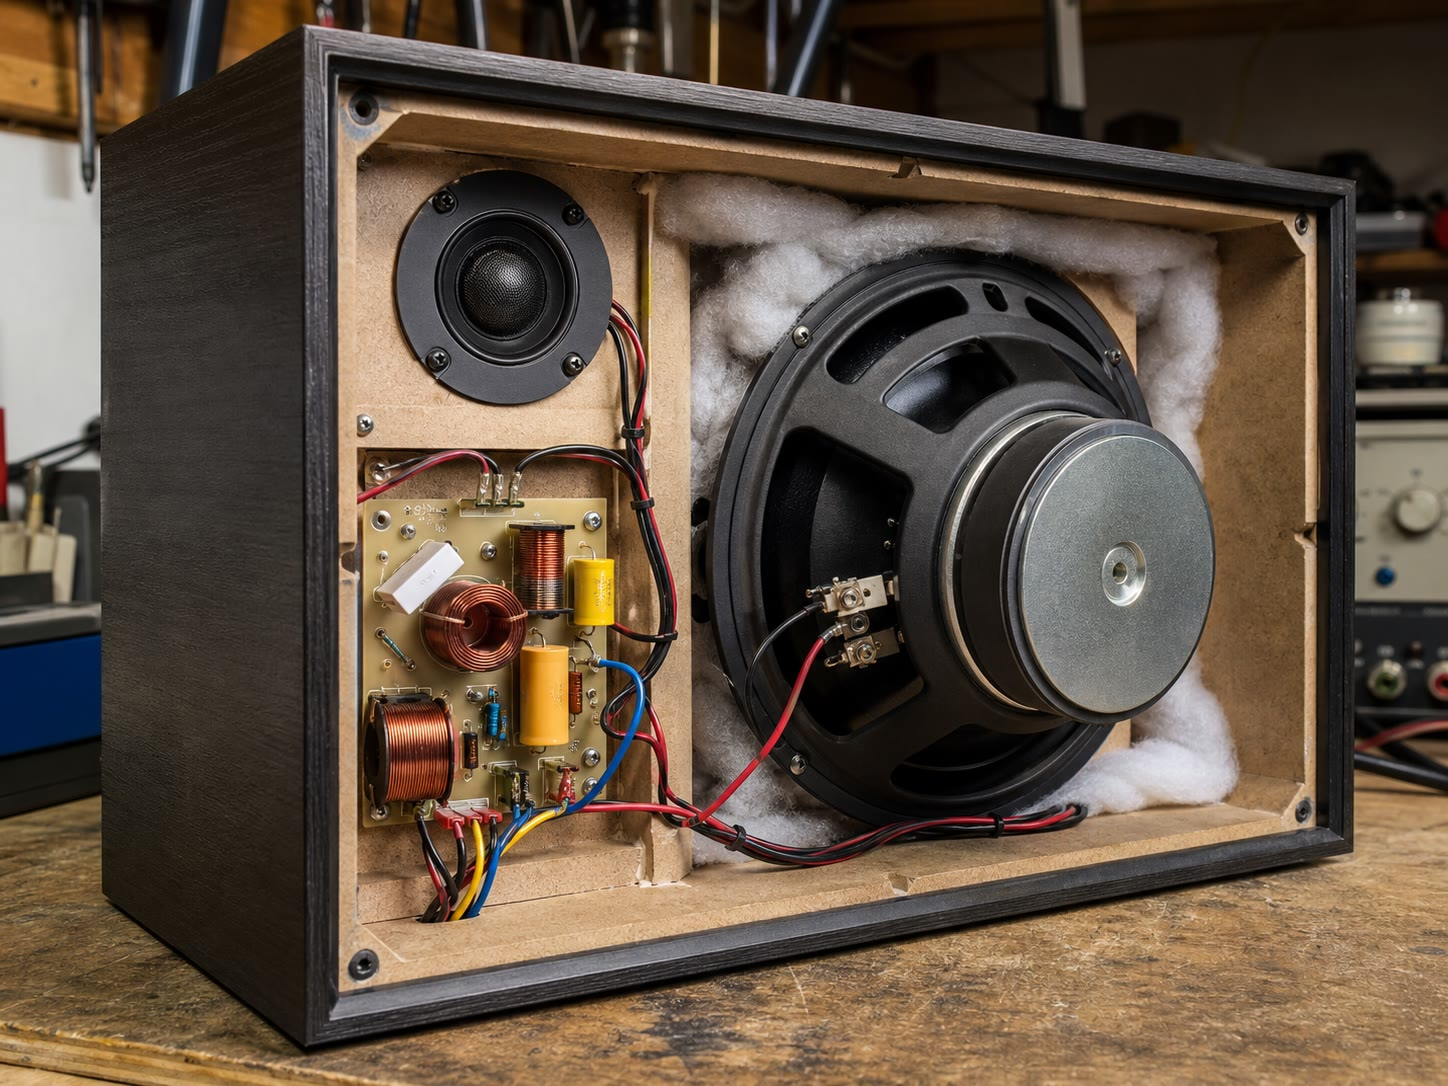
\includegraphics[width=0.50\linewidth]{images/book3/ai/b3-09-loudspeaker-crossover.jpg}

{\small In een tweewegluidspreker: de spoelen en condensatoren van het wisselfilter zijn de laag- en \omterm{prop:b1:filters-transfer-functions:highpass1}{hoogdoorlaatfilters} die de bas naar de woofer en de hoge tonen naar de tweeter sturen.}
\end{omfigure}

\section{Probleem: Het wisselfilter van een luidspreker}

\begin{problem}[{Weekendopgave --- een woofer, een tweeter, een spoel en een
condensator: hoe een passief wisselfilter de muziek verdeelt, waarom het
eenvoudigste model bas in de tweeter laat lekken, en wat een echte spreekspoel met
het ontwerp doet}]
\label{pb:b1:filters-transfer-functions:1}
De woofer en de tweeter worden eerst als zuivere weerstanden
$R = \qty{8.0}{\ohm}$ gemodelleerd. De versterker is een ideale \omterm{def:b1:dc-circuits:sources}{spanningsbron}
$\underline U_e$. De scheidingsfrequentie is $f_c = \qty{2.0}{kHz}$.

\medskip
\noindent\textbf{Deel I --- Wisselfilter van de eerste orde.}
De woofer wordt gevoed via een spoel $L$ in serie, de tweeter via een
condensator $C$ in serie.
\begin{enumerate}
  \item Definieer de \omterm{def:b1:filters-transfer-functions:H}{overdrachtsfunctie} van elke tak (\omterm{def:b1:dc-circuits:voltage}{spanning} over de
        luidspreker gedeeld door $\underline U_e$) en de \omterm{def:b1:filters-transfer-functions:H}{versterking} in \omterm{def:b1:filters-transfer-functions:bode}{decibel}.
  \item Toon aan dat de woofertak een laagdoorlaat van de eerste orde is en geef
        haar \omterm{def:b1:filters-transfer-functions:bode}{afsnijfrequentie} $\omega_c$ in termen van $R$ en $L$.
  \item Bereken $L$ voor $f_c = \qty{2.0}{kHz}$.
  \item Toon aan dat de tweetertak een hoogdoorlaat van de eerste orde is; geef
        $\omega_c$ en bereken $C$.
  \item Geef de \omterm{def:b1:filters-transfer-functions:H}{versterking} van elke luidspreker in \omterm{def:b1:filters-transfer-functions:bode}{decibel} bij $f_c$, bij \qty{200}{Hz}
        en bij \qty{20}{kHz}.
  \item Toon aan dat $G_L^2 + G_H^2 = 1$ bij elke frequentie. Wat betekent
        dat voor het vermogen dat aan de versterker wordt onttrokken?
  \item Geef de fase van elke tak bij $f_c$; hoeveel verschillen de \omterm{def:b1:dc-circuits:voltage}{spanningen}
        over de twee luidsprekers daar in fase?
  \item Wat zijn de hellingen van de twee responsies, in dB per octaaf, ver
        van $f_c$?
\end{enumerate}

\medskip
\noindent\textbf{Deel II --- Wisselfilter van de tweede orde.}
De woofer wordt nu gevoed via een spoel $L$ in serie met een condensator $C$
parallel aan de luidspreker.
\begin{enumerate}[resume]
  \item Toon aan dat $\underline H = 1/(1 - LC\omega^2 + jL\omega/R)$.
  \item Identificeer $\omega_0$ en $Q$ in termen van $L$, $C$, $R$.
  \item Toon voor $Q = 1/\sqrt2$ aan dat $G = 1/\sqrt{1 + (\omega/\omega_0)^4}$
        en dat de \omterm{def:b1:filters-transfer-functions:H}{versterking} \qty{-3}{dB} is bij $\omega_0$.
  \item Bereken $L$ en $C$ voor $f_0 = \qty{2.0}{kHz}$ en $Q = 1/\sqrt2$.
  \item Bereken de \omterm{def:b1:filters-transfer-functions:H}{versterking} in \omterm{def:b1:filters-transfer-functions:bode}{decibel} bij \qty{4}{kHz} en \qty{8}{kHz};
        leid de helling in dB per octaaf af.
  \item De tweetertak verwisselt de rollen van $L$ en $C$ ($C$ in serie,
        $L$ parallel): schrijf haar \omterm{def:b1:filters-transfer-functions:H}{overdrachtsfunctie} op zonder nieuwe
        berekening.
  \item Bereken de fase van elke tak bij $f_0$. Wat moet er met de bedrading
        van de tweeter gebeuren, en waarom?
\end{enumerate}

\medskip
\noindent\textbf{Deel III --- Muziek door het wisselfilter.}
\begin{enumerate}[resume]
  \item Een cellotoon van \qty{220}{Hz} draagt harmonischen tot de twintigste.
        Welke harmonischen gaan bij het wisselfilter van de eerste orde
        overwegend naar de tweeter?
  \item Wat gebeurt er met de negende harmonische?
  \item Als testsignaal wordt een blokgolf van \qty{1.0}{kHz} gebruikt. Geef met
        het wisselfilter van de eerste orde de \omterm{def:b1:filters-transfer-functions:H}{versterking} van elke tak voor haar
        grondtoon en haar derde en vijfde harmonische.
  \item De versterker krijgt per ongeluk een gelijkspanningsoffset van \qty{1}{V}. Welke
        luidspreker is beschermd, en waardoor?
  \item Welke fractie van de \omterm{def:b1:dc-circuits:voltage}{spanning} en van het vermogen van een toon van
        \qty{500}{Hz} bereikt met het wisselfilter van de eerste orde de tweeter?
        Idem met dat van de tweede orde. Waarom telt dit voor het
        voortbestaan van de tweeter?
\end{enumerate}

\medskip
\noindent\textbf{Deel IV --- Een echte spreekspoel.}
De woofer is in werkelijkheid $R = \qty{8.0}{\ohm}$ in serie met een zelfinductie
$L_{vc} = \qty{0.50}{mH}$ van de spreekspoel.
\begin{enumerate}[resume]
  \item Bereken de \omterm{def:b1:sinusoidal-impedance:impedance}{impedantie} (modulus) van de woofer bij \qty{2}{kHz} en bij
        \qty{8}{kHz}.
  \item Herbereken met deze \omterm{def:b1:sinusoidal-impedance:impedance}{impedantie} de \omterm{def:b1:filters-transfer-functions:H}{woofer-versterking} van de eerste orde bij
        \qty{2}{kHz} en \qty{8}{kHz} en vergelijk met de ideale
        \qty{-3}{dB} en \qty{-12.3}{dB}. Wat is er met het afvallen gebeurd?
  \item Een ``Zobel-netwerk'' --- $R_z = R$ in serie met $C_z =
        L_{vc}/R^2$ --- wordt parallel aan de woofer geschakeld. Toon aan
        dat de combinatie zich bij elke frequentie als een zuivere weerstand $R$
        gedraagt, en bereken $C_z$.
  \item De versterker levert \qty{50}{W} in \qty{8}{\ohm}: welke effectieve
        \omterm{def:b1:dc-circuits:voltage}{spanning} is dat, en welk vermogen ontvangt elke luidspreker bij
        $f_c$ (wisselfilter van de eerste orde)? Hoeveel bereikt bij \qty{500}{Hz}
        de tweeter?
  \item Vat de afwegingen samen: helling, fase, aantal onderdelen,
        bescherming van de tweeter en de noodzaak van een Zobel-netwerk.
\end{enumerate}
\end{problem}
